%\documentclass[a4paper,10pt]{book}

%Use the following for font size 8 or 9, as 10 is the minimum provided normally
\documentclass[9pt]{extbook}

%Preferred font and spacing
\linespread{1.3}
%\usepackage{lmodern}
\usepackage{kpfonts}

%Compilers
\usepackage[utf8]{inputenc}
\usepackage[english]{babel}

%Graphics
\usepackage{xcolor}
\usepackage{graphicx}

%Math
\usepackage{amsmath}
\usepackage{amssymb}
\usepackage{enumitem}
\usepackage{caption}
\usepackage{physics}
\usepackage{amsthm}
\usepackage{mathtools}
\usepackage[xcolor]{mdframed}

%Math shortcuts 
\newcommand{\R}{\mathbb{R}}
\newcommand{\C}{\mathbb{C}}
\newcommand{\F}{\mathbb{F}}
\newcommand{\M}{\mathcal{M}}
\renewcommand{\P}{\mathcal{P}}
\renewcommand{\L}{\mathcal{L}}
\DeclareMathOperator{\Span}{span}
\DeclareMathOperator{\Dim}{dim}
\DeclareMathOperator{\Codim}{codim}
\DeclareMathOperator{\Range}{range}
\DeclareMathOperator{\Rank}{rank}
\DeclareMathOperator{\Null}{null}
\DeclareMathOperator{\Ker}{ker}
\let \Trace \relax %\Trace is already defined so resetting
\DeclareMathOperator{\Trace}{tr} 
\DeclareMathOperator{\Det}{det}
\newcommand{\A}{\alpha}
\newcommand{\B}{\beta}

%Augmented matrices
\makeatletter
\renewcommand*\env@matrix[1][*\c@MaxMatrixCols c]{%
   \hskip -\arraycolsep
   \let\@ifnextchar\new@ifnextchar
   \array{#1}}
\makeatother

%Remove auto-indentation
\setlength{\parindent}{0cm}

%Reducing margin
\usepackage[margin=2cm]{geometry}

%Change section, subsection 
\usepackage{titlesec}
\titleformat{\section}
	{\huge\bfseries}{}
	{0em}{}
\titleformat{\subsection}
	{\LARGE\bfseries}{}
	{0em}{}

%Header, footer
\usepackage{fancyhdr}
\pagestyle{fancy}
\fancyhf{}
\rhead{\leftmark}
\cfoot{\thepage} 
\renewcommand{\headrulewidth}{0pt}

%Table of Contents 
\usepackage{hyperref}
\hypersetup{
    colorlinks,
    citecolor=black,
    filecolor=black,
    linkcolor=blue,
    urlcolor=blue
}

\newcounter{exercise}
\newcounter{problem}[exercise]

\newcommand{\exercise}{
	\stepcounter{exercise} 
	\subsection*{Exercise \thechapter.\theexercise} 
}




\title{Notes and Solutions for Nielsen and Chuang's \textit{Quantum Computation and Quantum Information}}
\date{2019}
\author{Warren Alphonso}

\begin{document}

\frontmatter 
\let\cleardoublepage\clearpage 
\maketitle
\tableofcontents

\mainmatter

\chapter{Introduction and overview}

\section{Notes}

``Instead of looking at quantum systems purely as phenomena to be explained..., they looked at them as systems that can be \textit{designed}...No longer is the quantum world taken merely as presented, but instead it can be \textit{created}." 

\subsection{Bloch Spheres}

For a complex number $z = x + iy$, where $x$ and $y$ are real, we can write 
$$\abs{z}^{2} = z^{*} z = (x - iy)(x + iy) = x^{2} + y^{2}$$

Using the polar representation gives us $z = r(\cos \theta + i \sin \theta)$. Substituting Euler's identity ($e^{i \theta} = \cos \theta + i \sin \theta$) results in 
$$ z = re^{i \theta}$$

We know qubits have complex amplitudes, so we can write
$$\ket*{\psi} = r_{\A} e^{i \theta_{\A}} \ket*{0} + r_{\B} e^{i \theta_{\B}} \ket*{1}$$
where all four variables are real. 

It turns out the term $e^{i \gamma}$ doesn't affect the probabilities $\abs{\A}^{2}$ or $\abs{\B}^{2}$:
$$ \abs{e^{i \gamma} \A}^{2} = (e^{i \gamma} \A)^{*} (e^{i \gamma} \A) = (e^{-i \gamma} \A^{*})(e^{i \gamma} \A) = \A^{*} \A = \abs{\A}^{2}$$
so we can multiply by $e^{-i \theta_{\A}}$ to get 
$$\ket*{\psi} = r_{\A} \ket*{0} + r_{\B} e^{i \theta} \ket*{1}$$
with three real parameters: $r_{\A}$, $r{\B}$, and $\theta = \theta_{\B} - \theta_{\A}$. 

Switching back to Cartesian coordinates and recalling the normalization condition, we have 
$$
\begin{aligned}
\abs{r_{\A}}^{2} + \abs{x + iy}^{2} &= r_{\A}^{2} + (x - iy)(x + iy) \\
&= r_{\A}^{2} + x^{2} + y^{2} = 1
\end{aligned}
$$
which is the equation for a sphere. Renaming $r_{\A}$ as $z$, we can use the identities
$$
\begin{aligned}
x &= r \sin \theta \cos \phi \\
y &= r \sin \theta \sin \phi \\
z &= r \cos \theta
\end{aligned}
$$
and after subbing in $r = 1$, we can write 
$$
\begin{aligned}
\ket*{\psi} &= z \ket*{0} + (x + iy) \ket*{1} \\
&= \cos \theta \ket*{0} + \sin \theta (\cos \phi + i \sin \phi) \ket*{1} \\
&= \cos \theta \ket*{0} + e^{i \phi} \sin \theta \ket*{1}
\end{aligned}
$$

Notice that $\theta =0 \rightarrow \ket*{\psi} = \ket*{0}$ and $\theta = \frac{\pi}{2} \rightarrow \ket*{\psi} = e^{i \phi} \ket*{1}$, which suggests that $0 \leq \theta \leq \frac{\pi}{2}$ generates all superpositions. In fact, one can easily check that plugging in $\theta' = \pi - \theta$ and $\phi' = \phi + \pi$ (the opposite point on the sphere) results in $-\ket*{\psi}$. Since the lower hemisphere of the sphere differs only by a phase factor of -1, we can choose to only consider the upper hemisphere. 

To map points in the upper hemisphere onto a sphere, we can write 
$$\ket*{\psi} = \cos \frac{\theta}{2} \ket*{0} + e^{i \phi} \sin \frac{\theta}{2} \ket*{1}$$
where $0 \leq \theta \leq \pi$ and $0 \leq \phi \leq 2\pi$. 

{
\centering 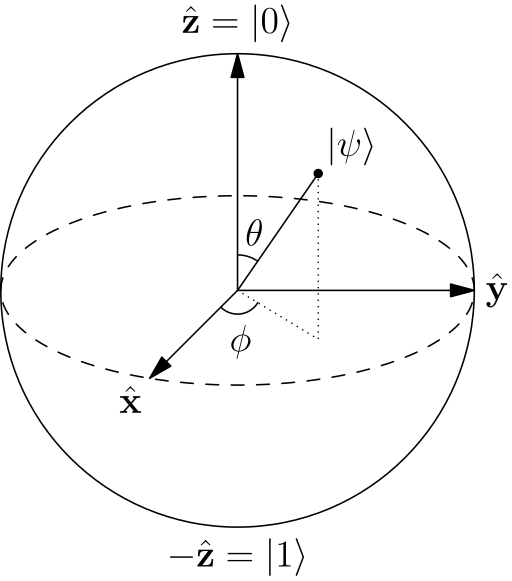
\includegraphics[width=.3\linewidth]{ch1/bloch.png}\par }

The poles represent classical states. When a qubit is measured, it has higher probability of collapsing to the pole it's closer to. This representation makes it clear that the Pauli Z gate results in only a \textit{phase change} because it does not affect the state the qubit will collapse to.\footnote{Image from \href{http://akyrillidis.github.io/notes/quant_post_7}{Anastasios Kyrillidis's notes}.} Now that we've derived Bloch spheres, there are two key properties we must understand:

\begin{enumerate}
	\item \textit{Orthogonality of opposite points:} Let $\ket*{\psi} = \cos \frac{\theta}{2} \ket*{0} + e^{i \phi} \sin \frac{\theta}{2} \ket*{1}$, and let $\ket*{\varphi}$ the opposite point on the Bloch sphere,
$$\ket*{\varphi} = \cos \Big( \frac{\pi - \theta}{2} \Big) \ket*{0} + e^{i(\phi + \pi)} \sin \Big( \frac{\pi - \theta}{2} \Big) \ket*{1} = \cos \Big( \frac{\pi - \theta}{2} \Big) \ket*{0} - e^{i \phi} \sin \Big( \frac{\pi - \theta}{2} \Big) \ket*{1}$$
Using the identity $\cos(a + b) = \cos a \cos b - \sin a \sin b$, we get
$$(\varphi, \psi) = \cos \Big( \frac{\theta}{2} \Big) \cos \Big( \frac{\pi - \theta}{2} \Big) - \sin \Big( \frac{\theta}{2} \Big) \sin \Big( \frac{\pi - \theta}{2} \Big) = \cos \Big( \frac{\pi}{2} \Big) = 0$$

	\item \textit{Rotations:} The Pauli X, Y, and Z gates are so-called because when exponentiated they yield rotation operators, which rotate the Bloch vector ($\sin \theta \cos \phi$, $\sin \theta \sin \phi$, $\cos \theta$) about the $x$, $y$, and $z$ axes. For example, the exponentiated Pauli X gate is
	$$R_{X} (\theta) = e^{-i\theta X / 2}$$
The exponentiated Pauli Y and Z gates are similarly defined. 

To understand this, note that in the special case where $A^{2} = I$ (which holds for all the Pauli matrices), 
$$
\begin{aligned}
e^{i \theta A} &= I + i\theta A - \frac{\theta^{2} I}{2!} - i \frac{\theta^{3} A}{3!} + \frac{\theta^{4} I}{4!} + i \frac{\theta^{5} A}{5!} + \cdots \\
&= \Big( 1 - \frac{\theta^{2}}{2!} + \frac{\theta^{4}}{4!} + \cdots \Big) I + i \Big( \theta - \frac{\theta^{3}}{3!} + \frac{\theta^{5}}{5!} + \cdots \Big) A \\
&= \cos (\theta) I + i \sin (\theta) A
\end{aligned}
$$

Now we can exponentiate the Pauli X gate as 
$$R_{X} (\theta) = e^{-i \theta X / 2} = \cos \frac{\theta}{2} I - i \sin \frac{\theta}{2} X = \begin{bmatrix}
\cos \frac{\theta}{2} & -i \sin \frac{\theta}{2} \\
-i \sin \frac{\theta}{2} & \cos \frac{\theta}{2}
\end{bmatrix}$$

Let's consider $R_{X}( \pi)$, 
$$R_{X} (\pi) = \begin{bmatrix}
\cos \frac{\pi}{2} & -i \sin \frac{\pi}{2} \\
-i \sin \frac{\pi}{2} & \cos \frac{\pi}{2}
\end{bmatrix} = \begin{bmatrix}
0 & -i \\
-i & 0
\end{bmatrix} = -iX$$
This is a 180 degree rotation across the x-axis since we swap amplitudes and the phase changes.\footnote{Most of this section is from \href{http://www.vcpc.univie.ac.at/~ian/hotlist/qc/talks/bloch-sphere.pdf}{Ian Glendinning's talk}.} \textbf{Todo:} Need an actual reason for why. 
\end{enumerate}

\subsection{Why must quantum gates be unitary?}

For a quantum state $\ket{\psi} = \A \ket{0} + \B \ket{1}$, we know $\abs{\A}^{2} + \abs{\B}^{2} = 1$ must be true. Another way of writing this is $(\ket{\psi}, \ket{\psi}) = 1$. This must also be true after the application of a quantum gate $U$. Thus, we have 
$$
\begin{aligned}
1 &= (U \ket{\psi}, U \ket{\psi}) = (\ket{\psi}, \ket{\psi}) \\
&= (U^{\dagger} U \ket{\psi}, \ket{\psi}) = (\ket{\psi}, \ket{\psi})
\end{aligned}
$$
which means $U^{\dagger}U = I$ is a fundamental constraint on quantum gates. 

\subsection{Decomposing single qubit operations}

Move to section 4.2 according to Box 1.1 on p20. 

\subsection{What does the matrix representation of a quantum gate mean?}

$$U_{CN} = \begin{bmatrix}
1 & 0 & 0 & 0 \\
0 & 1 & 0 & 0 \\
0 & 0 & 0 & 1 \\
0 & 0 & 1 & 0
\end{bmatrix}$$

This $U_{CN}$ gate acts on two qubits, so it is a transformation on basis vectors $\ket*{0} \otimes \ket*{0}$, $\ket*{0} \otimes \ket*{1}$, $\ket*{1} \otimes \ket*{0}$, and $\ket*{1} \otimes \ket*{1}$. The columns tell us that an input of the third basis vector, $\ket*{1} \otimes \ket*{0}$, will output the fourth basis vector, $\ket*{1} \otimes \ket*{1}$. 

\textbf{Todo:} What does this say about superpositions?

\subsection{Why must quantum gates be reversible?}
Since quantum gates are unitary, we know $U^{\dagger} U = I$, which means quantum gates are invertible, and the inverse is also a quantum gate because it is unitary. 

One implication of this is that classical gates like \textsc{XOR} and \textsc{NAND} have no quantum cousins because these gates are irreversible since they result in a loss of information. 

Well, technically, the Toffoli gate can be used to simulate \textsc{NAND} gates (and therefore all classical gates), but it can only do so because it explicitly preserves all input bits. 

\section{Solutions}

\exercise
2 evaluations. If we get the same value and guess the constant function, there's a 25\% chance it was the balanced function. 

\exercise 
If we could fully identify the state, we can just bitwise add our result to $\ket*{0}$ to get a clone of our original state. 

For the converse, if we had a device that could clone quantum states, we could continue cloning and measuring the clones to get an arbitrary level of accuracy of the original quantum state. 


\chapter{Introduction to quantum mechanics}

\section{Notes}

\subsection{Notation}

For distinct vectors in an orthonormal set, we can write $\braket*{i}{j} = \delta_{ij}$, where $\delta_{ij}$ is the Kronecker product and is 1 if $i = j$ and 0 if $i \neq j$. 

\subsection{Matrix - Linear Operator Congruence}

For a matrix to a be a linear operator, 
$$A \Big( \sum_{i} a_{i} \ket*{v_{I}} \Big) = \sum_{i} a_{i} A \ket*{v_{i}}$$
must be true. Note the LHS is the sum of vectors to which $A$ is applied which is certainly equal to the RHS. 

Now suppose $A: V \rightarrow W$ is a linear operator and that $V$ has basis $\ket*{v_{i}}, \cdots, \ket*{v_{m}}$ and $W$ has basis $\ket*{w_{i}}, \cdots, \ket*{w_{n}}$. Since we know the $k$th column of a $A$ will be its transformation of $\ket*{v_{k}}$, 
$$A \ket*{v_{j}} = \sum_{i} A_{ij} \ket*{w_{i}}$$
Note this is just saying $A \ket*{v_{j}}$ is equal to the $j$th column of $A$, and we can think of $\ket*{w_{i}}$ as the coordinates of the transformed vector. Thus, we can find the matrix representation of any linear operator by finding a matrix $A$ with entries specified by the above equation. 

\subsection{What's so special about the Pauli matrices?}

Things to look into: \begin{itemize}
\item they pop up in the Pauli equation 
\item they form a basis for the vector space of $2 \times 2$ Hermitian matrices. Hermitian matrices represent observables? Look at Wikipedia page
\end{itemize}

\subsection{What does the Completeness Relation say about matrices?}

I don't understand why $$\sum_{ij} \bra*{w_{j}} A \ket*{v_{i}} \ket*{w_{j}} \bra*{v_{i}}$$ implies $A$ has matrix element $\bra{w_{j}} A \ket*{v_{i}}$ in the $i$th column and $j$th row, with respect to input basis $\ket*{v_{i}}$ and output basis $\ket*{w_{j}}$. page 68. 


\section{Solutions}

\exercise
$$\begin{bmatrix}
1 \\
-1
\end{bmatrix} + \begin{bmatrix}
1 \\
2 
\end{bmatrix} - \begin{bmatrix}
2 \\
1
\end{bmatrix} = 0$$

\exercise
$$A = \begin{bmatrix}
0 & 1 \\
1 & 0
\end{bmatrix}$$ because $A\ket*{0}$ has coordinate 0 in $\ket*{0}$ and coordinate 1 in $\ket*{1}$. 

If we keep our input bases the same but reorder our output bases as $\ket*{1}$ and $\ket*{0}$, 
$$A = \begin{bmatrix}
1 & 0 \\
0 & 1
\end{bmatrix}$$

\exercise 
We know 
$$A \ket*{v_{i}} = \sum_{j} A_{ji} \ket*{w_{j}}$$
and 
$$B \ket*{w_{j}} = \sum_{k} B_{kj} \ket*{x_{k}}$$

Now we can write 
$$
\begin{aligned}
BA \ket*{v_{i}} = B ( A \ket*{v_{i}} ) = B \sum_{j} A_{ji} \ket*{w_{j}} &= \sum_{j} A_{ji} (B \ket*{w_{j}}) \\
&= \sum_{j} A_{ji} \sum_{k} B_{kj} \ket*{x_{k}} \\
&= \sum_{k} \sum_{j} B_{kj} A_{ji} \ket*{x_{k}} \\
&= \sum_{k} (BA)_{ki} \ket*{x_{k}}
\end{aligned}
$$
We know $\sum_{k} (BA)_{ki}$ is the matrix representation of operator $BA$, which the preceding step says is equal to $\sum_{k} \sum_{j} B_{kj} A_{ji}$, which is the matrix multiplication $BA$. 

\exercise 
For the same input and output basis, we want some $I$ such that 
$$I\ket*{v_{j}} = \sum_{i} I_{ij} \ket*{v_{i}} = \ket*{v_{j}}$$
which means $I_{ij} = 0$ for all $i \neq j$ and 1 otherwise. 

\exercise
For $\ket*{y}, \ket*{z_{i}} \in \C^{n}$ and $\lambda_{i} \in C$, 
$$
\begin{aligned}
\Big( \ket*{y}, \sum_{i} \lambda_{i} \ket*{z_{i}} \Big) &= \ket*{y}^{*} \sum_{i} \lambda_{i} \ket*{z_{i}} \\
&= \sum_{i} \lambda_{i} \ket*{y}^{*} \ket*{z_{i}} \\
&= \Big( \sum_{i} \lambda_{i}^{*} \ket*{z_{i}}^{*} \ket*{y} \Big)^{*}
\end{aligned}
$$
The second and third equalities demonstrate linearity in the second argument and $(\ket*{y}, \ket*{z}) = (\ket*{z}, \ket*{w})^{*}$. Finally, if $\ket*{w} = (w_{1}, \cdots, w_{n})$ where $w_{i} \in \C^{n}$, then
$$(\ket*{w}, \ket*{w}) = \sum_{i} w_{i}^{*} w_{i} = \sum_{i} \abs{w_{i}}^{2}$$
which proves the non-degeneracy and non-negativity condition. 

\exercise
$$
\begin{aligned}
\Big( \sum_{i} \lambda_{i} \ket*{w_{i}}, \ket*{v} \Big) &= \Big( \ket*{v}^{*}, \sum_{i} \lambda_{i}^{*} \ket*{w_{i}}^{*} \Big)^{*} \\
&= \sum_{i} \lambda_{i}^{*} \Big( \ket*{v}^{*}, \ket*{w_{i}}^{*} \Big)^{*} \\
&= \sum_{i} \lambda_{i}^{*} \Big( \ket*{w_{i}}, \ket*{v} \Big)
\end{aligned}
$$

\exercise
$$(\ket*{w}, \ket*{v}) = \begin{bmatrix}
1 & 1
\end{bmatrix} \begin{bmatrix}
1 \\
-1
\end{bmatrix} = 1 - 1 = 0$$
To normalize, divide each vector by $\sqrt{2}$. 

\exercise
Since at each step, we divide by the norm of the vector being added, the set is orthonormal. The set is a basis because at step $i$, we add the basis vector $\ket*{w_{i}}$ but subtract out the portion that was already in $\Span( \ket*{v_{1}}, \cdots, \ket*{v_{i-1}})$, so we still end up spanning the full vector space. 

\exercise
$$\sigma_{x} = \ket*{1} \bra*{0} + \ket*{0} \bra*{1} $$
$$\sigma_{y} = i \ket*{1} \bra*{0} - i \ket*{0} \bra*{1}$$
$$\sigma_{z} = \ket*{0} \bra*{0} - \ket*{1} \bra*{1}$$

\exercise
$$
\begin{aligned}
\ket*{v_{j}} \bra*{v_{k}} &= I \ket*{v_{j}} \bra*{v_{k}} I \\
&= \sum_{a} \ket*{v_{a}} \braket*{v_{a}}{v_{j}} \sum_{b} \braket*{v_{k}}{v_{b}} \bra*{v_{b}} \\
&= \sum_{a, b} \delta_{aj} \delta_{kb} \ket*{v_{a}} \bra*{v_{b}}
\end{aligned}
$$
so the element $(\ket*{v_{j}} \bra*{v_{k}})_{ab} = \delta_{aj} \delta_{kb}$. 

\exercise
Each of the Pauli matrices has eigenvalues $\pm 1$. 

For $\sigma_{x}$, 
$$\sigma_{x+} = \begin{bmatrix}
1 \\
1
\end{bmatrix} \text{ and } \sigma_{x-} = \begin{bmatrix}
-1 \\
1
\end{bmatrix}$$

For $\sigma_{y}$, 
$$\sigma_{y+} = \begin{bmatrix}
1 \\
i
\end{bmatrix} \text{ and } \sigma_{y-} = \begin{bmatrix}
i \\
1
\end{bmatrix}$$

For $\sigma_{z}$, 
$$\sigma_{z+} = \begin{bmatrix}
1 \\
0
\end{bmatrix} \text{ and } \sigma_{z-} = \begin{bmatrix}
0 \\
1
\end{bmatrix}$$
The diagonalization easily follows. 

\exercise
The characteristic equation is $(1 - \lambda)^{2}$, so we have eigenvalue $1$. Solving $(A - 1I)\ket*{v} = 0$ gives us $\ket*{v} = \begin{bmatrix}
0 \\
1
\end{bmatrix}$. Our diagonal form should be $$A = \ket*{v} \bra*{v} = \begin{bmatrix}
0 & 0 \\
0 & 1
\end{bmatrix} \neq \begin{bmatrix}
1 & 0 \\ 
1 & 1
\end{bmatrix}$$

\exercise
$$(\ket*{w} \bra*{v})^{\dagger} = \bra*{v}^{\dagger} \ket*{w}^{dagger} = \ket*{v} \bra*{w}$$

\exercise
Since we know $(a + b)^{\dagger} = a^{\dagger} + b^{\dagger}$, so $$\Big( \sum_{i} a_{i} A_{i} \Big)^{\dagger} = \sum_{i} \Big( a_{i} A_{i} \Big)^{\dagger} = \sum_{i} \Big( a_{i}^{*} A_{i}^{\dagger} \Big)$$

\exercise
$$(\ket*{v}, A\ket*{w}) = (A^{\dagger} \ket*{v}, \ket*{w}) = \Big(\ket*{v}, (A^{\dagger})^{\dagger} \ket*{w} \Big)$$
since this holds for all $\ket*{v}, \ket*{w}$, $A = (A^{\dagger})^{\dagger}$. 

\exercise
$$P^{2} = \sum_{i} \ket*{i} \bra*{i} \sum_{j} \ket*{j} \bra*{j} = \sum_{ij} \ket*{i} \braket*{i}{j} \bra*{j} = \sum_{ij} \delta_{ij} \ket*{i} \bra*{j}$$

Intuitively, projecting some $\ket*{v} \in P $ wouldn't change $\ket*{v}$ at all. 

\exercise
Since $A$ is normal, we can diagonalize it. If the eigenvalues are all positive, then the adjoint of this diagonal matrix of eigenvalues equals itself. If $A$ is Hermitian, then so is its diagonal form. The adjoint of a diagonal matrix consists of the conjugates of its diagonal entries, so if $A = A^{\dagger}$, then the diagonal entries (eigenvalues) must all be positive. 


\end{document}